\documentclass[10pt]{article}
\usepackage{graphicx}

\title{Converting RMS topography to a 2D spatial map}
\author{Claire}

\begin{document}
\maketitle

\section{Fit baseline spectrum}

A 2D convection simulation results in a profile of the surface dynamic topography. A discrete cosine transform of this profile produces a 1D power spectral density, $\phi^{1D}_0$ as a function of wavenumber, $k$ (figure \ref{fig:aspect_spectrum}). This spectrum has a root mean square topography rms$_0$.

In log-log space this spectrum is approximately linear from $k_{min}$, corresponding to a wavelength somewhere near twice the layer depth, to $k_{max}$, corresponding to a wavelength 6--7 times larger than the boundary layer thickness. At wavenumbers below $k_{min}$, the spectrum rolls off to a constant value. Therefore we fit a constant slope between $k_{min}$ and $k_{max}$, and assign a value of $\phi^{1D}_0(k_{min})$ wherever $k < k_{min}$. We remove spherical harmonic degrees $l \le 1$, where $l = kR - 0.5$. We assume a planet radius $R = 2$; i.e., a core radius fraction of 0.5. We interpolate this fitted function such that it has a discrete value at each $l$.

\begin{figure}[h]
\centering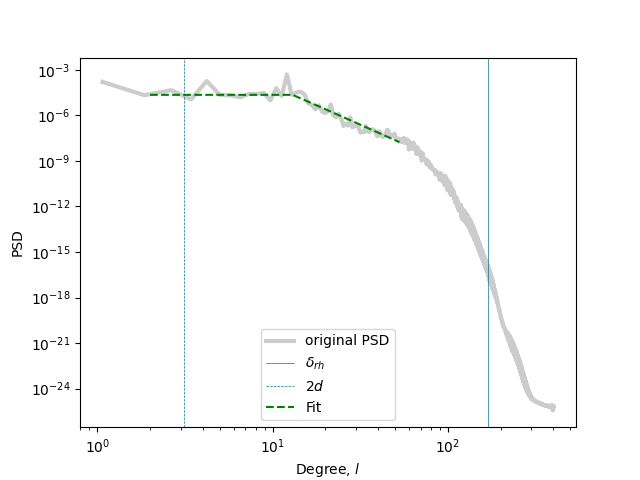
\includegraphics[width=1\linewidth]{fit.png}
\caption{The baseline spectrum fit in nondimensional units. \label{fig:aspect_spectrum}}
\end{figure}

\section{Get spherical harmonic coefficients}

We will use the {\tt pyshtools.SHCoeffs.from{\_}random()} function to obtain a set of spherical harmonic coefficients consistent with $\phi^{1D}_0$. However, this function takes a power per $l$ (dimensional units m$^2$), to which we must convert  $\phi^{1D}_0$ (dimensional units m$^2$~m).

\subsection{Convert from 1D power spectral density}

First we find the effective 2D power spectral density assuming radial symmetry, $\phi^{2D}_{iso}$ (dimensional units m$^2$~m$^2$), which corresponds to our 1D spectrum:
\begin{equation}
\phi^{2D}_{iso} = \frac{1}{k} \phi^{1D}_0.
\end{equation}
These should have approximately the same total power by Parseval's theorem in the relevant dimensions;
\begin{equation}
\frac{1}{4\pi^2}\int\left(\phi^{2D}_{iso}2\pi k \; \rm{d}k \right) = \frac{1}{2\pi}\int\left(\phi^{1D}_0 \; \rm{d}k \right).
\end{equation}
Then the total power per $l$ is:
\begin{equation}
S_l = \frac{\phi^{2D}_{iso} \left(2 l + 1\right)}{4 \pi R^2}.
\end{equation}
Note that the power per $lm$,
\begin{equation}
S_{lm} = \frac{S_l}{2l + 1},
\end{equation}
has the same units as $\phi^{2D}_{iso}$.

\subsection{Optional rms shift} If we are seeking a spatial map of a hypothetical spectrum other than $\phi^{1D}_0$ (i.e., different Rayleigh number), at this stage we take advantage of the fact that dynamic topography spectra appear to have consistent shapes across Rayleigh numbers, and multiply $S_l$ by the rms ratio squared, 
\begin{equation}
\bar{S_l} = S_l \left(\frac{\rm{rms}_1}{\rm{rms}_0}\right)^2,
\end{equation}
where rms$_1$ refers to the desired rms of the new spectrum. Otherwise, rms$_1$ = rms$_0$. Note that we are still working in nondimensional units.

\subsection{Generate random spherical harmonic coefficients} We can now obtain our set of random coefficients via \\ {\tt pyshtools.SHCoeffs.from{\_}random(Sl, normalization=`ortho')}. Setting the normalisation at this stage means that all class function calls will use the same normalisation. As a a test, we can look at the power per $l$, $S_l^{\rm rand}$ and power per $lm$, $S_{lm}^{\rm rand}$ of these coefficients using the {\tt spectrum(unit)} function from the {\tt pyshtools.SHCoeffs} class. We expect that $S_{lm}^{\rm rand}$ looks like $\phi^{2D}_{iso}$ and
\begin{equation} \label{eq:rand_rms_check}
\frac{1}{2\pi}\int\left(4 \pi R^2 S_{lm}^{\rm rand} k \; \rm{d}k \right) \approx \left({\rm rms_1}\right)^2.
\end{equation}
Figure \ref{fig:test_spectra} compares these fitted and randomised power spectra and spectral densities.

\begin{figure}[h]
\centering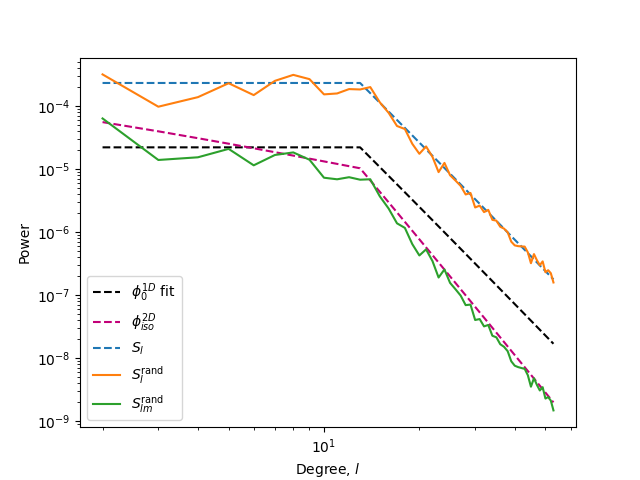
\includegraphics[width=1\linewidth]{random_spectra.png}
\caption{Power spectra and spectral densities (dashed lines), with their randomly generated equivalents (solid lines), on the same axes. \label{fig:test_spectra}}
\end{figure}

\section{2D grid expansion}

After verifying (\ref{eq:rand_rms_check}), we use the {\tt expand()} function from the {\tt pyshtools.SHCoeffs} class to find the topography $h$ as a function of latitude and longitude. We find that the total power from this grid is approximately equal to the total power of $S_{lm}^{\rm rand}$ (and $S_l$) from Parseval's theorem in 2D,
\begin{equation}
\frac{\sum h^2}{ N_{\rm cells}} \approx \frac{1}{4\pi^2}\int\left(4 \pi R^2 S_{lm}^{\rm rand} 2\pi k \; \rm{d}k \right),
\end{equation}
which is greater than rms$_1$. \textbf{Now I am not sure how to ``convert" this $h$ such that it is consistent with ${\rm rms}_1$, because it is not.} I read that pseudo-1D and 2D radially symmetric PSDs would have rms off by $\pi/2$ (Jacobs et al., 2017), but the discrepancy is greater than this.

\subsection{Dimensionalisation}

At this point we would dimensionalise the spatial domain topography by multiplying it with $d \Delta T \alpha$ (values from the parameterised convection model). For the case I tested, doing this at face value---taking $h$ as above---results in a dimensional rms at least twice as large as the dimensionalised rms$_1$.\\ \\ \\

\noindent References \\

\noindent Jacobs, Tevis D. B., Till Junge, and Lars Pastewka. ‘Quantitative Characterization of Surface Topography Using Spectral Analysis’. Surface Topography: Metrology and Properties 5, no. 1 (27 January 2017): 013001. https://doi.org/10.1088/2051-672X/aa51f8.


\end{document}